\section{T3}

Establish the minimum cost spanning tree of the given map graph with Krustal's algorithm. The Krustal's algorithm holds the idea that to make the cost of spanning a tree in graph minimum, we take the smaller edges as much as possible.

\subsection{Code Designs}
\subsubsection*{a. Implement the generic \textbf{GenMST}}
In detail, the Krustal's algorithm can be written in the following executing order:
\begin{itemize}
    \item Sort all the edges in ascending order to a candidate sequence, initiate the graph to empty.
    \item Select the current shortest edge (if there is multiple choices, it's arbitrary), check if adding this edge to the graph conflict with the tree properties (say, result in a cycle in the graph). If so, roll back (say, don't choose this edge). Whether the edge conflicts or not, erase it from the candidate sequence. 
    \item Repeat the above step until the number of edges in the graph equals to the number of nodes in our given map minus 1 (property of a spanning tree). And we can ensure that the candidate sequence can provide enough candidate edges until we generate the spanning tree.
\end{itemize}

Above is the algorithm and also the backbone of our functions. Then introduce the interfaces.

\mintinline{c++}{void EdgeSort(std::vector<weighted_edge_type> &w_edges);} \newline
We use \verb|EdgeSort| in \verb|include\edges.h|, which is a quite version of \verb|MinHeapSort| (the original version is verbose and will give the detailed intermediate steps which is not necessary here)

\mintinline{c++}{std::vector<connected_graph_type> connected_components(}\newline
\mintinline{c++}{                     std::vector<weighted_edge_type> w_edges);}\newline
This function in \verb|include\MST.h| divise the current graph to connected components, and it will be easier to check if there is a cycle in a connected graph by simply calculating the number of nodes and that of edges.

\mintinline{c++}{std::vector<weighted_edge_type> GenMST(}\newline \mintinline{c++}{                     std::vector<weighted_edge_type> w_edges);}\newline
This function in \verb|include\MST.h| executes the whole algorithm described before

\subsection{QAs}
\subsubsection*{b and c. Result of Krustal's algorithm}
\begin{verbatim}
================ Test for GenMST ================
MST including edges:
[BJ <--9--> TJ] [LZ <--84--> XA] [LZ <--85--> CD] [CD <--86--> KM] 
[BJ <--88--> SY] [XA <--90--> BJ] [GZ <--91--> FZ] [SH <--92--> FZ] 
[TJ <--93--> SH] [XA <--94--> WH] [LS <--110--> CD] [WL <--120--> LS] 
================ Test for GenMST ================
MST weights:
1042
\end{verbatim}
There are in all $12$ routes, and the minimum cost is $1042$

\subsubsection*{d. Draw the established MST}
The established MST is: \newline
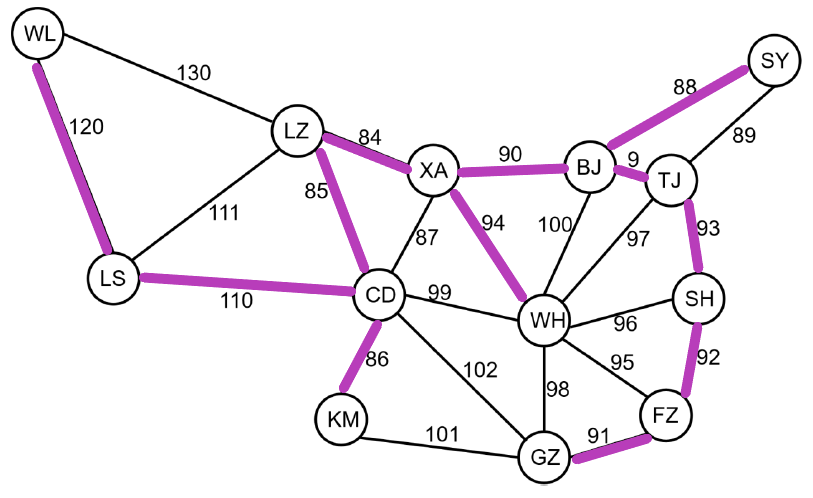
\includegraphics[width=4in]{content/mst.png}


\subsubsection*{e. MST with binary tree}
When \verb|WH| is chosen as the root node, the MST tree can be spanned in this order: \newline
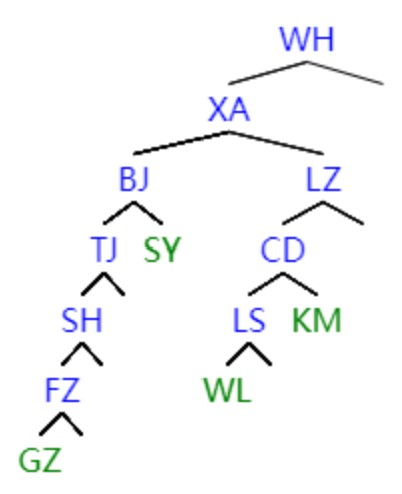
\includegraphics[width=1.5in]{content/bin.jpg}

In this case the MST is a binary tree. 
We give the traverses of this tree:
\begin{itemize}
    \item Preorder: WH - XA - BJ - TJ - SH - FZ - GZ - SY - LZ - CD - LS - WL - KM
    \item Inorder: \ \ GZ - FZ - SH - TJ - BJ - SY - XA - WL - LS - CD - KM - LZ - WH
    \item Postorder: GZ - FZ - SH - TJ - SY - BJ - WL - LS - KM - CD - LZ - XA - WH
\end{itemize}

That's all for \textit{task 3}.